\documentclass[10pt,a4paper]{article}

\usepackage[utf8]{inputenc}
\usepackage[T1]{fontenc}
\usepackage[french,english]{babel}
\usepackage{blindtext}

\usepackage[hyphens]{url}
\usepackage{hyperref}
\DeclareUrlCommand\email{\urlstyle{rm}}

\usepackage[margin=2in]{geometry} % showframe
\usepackage{multicol}

\usepackage{graphicx}
\usepackage{xcolor}
\usepackage{amsmath}
\usepackage{amsthm}
\usepackage{amsfonts}
\usepackage{amssymb}
\usepackage{siunitx}
\usepackage{pdflscape}
%\usepackage[toc]{glossaries} % https://www.overleaf.com/learn/latex/Glossaries
%\usepackage{parskip} % empty line between paragraphs
\usepackage{listings}
\usepackage{float}
\usepackage{pmboxdraw}
\usepackage{textcomp} % for the apostrophe
\usepackage{float}

% hyperref setup
\definecolor{darkgreen}{RGB}{0,180,0}
\hypersetup{
    colorlinks = true,
    linkbordercolor = {white},
    linkcolor = red,
    anchorcolor = black,
    citecolor = darkgreen,
    filecolor = cyan,
    menucolor = black,
    runcolor = cyan,
    urlcolor = magenta
}

% Bib setup
\usepackage{csquotes} % Recommended by biblatex
\usepackage[style=numeric,sorting=none,backend=biber]{biblatex}
\addbibresource{references.bib} % The file containing our references, in BibTeX format

\title{Experiments on automation of formal verification of devices at the binary level}
\author{Thomas Lacroix --- \email{thomas.lacroix@insa-lyon.fr}\medskip\\
Département Informatique\\
INSA de Lyon}
\date{2018/2019}

\begin{document}

\newgeometry{margin=2cm}

\maketitle
\thispagestyle{empty}

{
\noindent Sous la responsabilité de :\\
Mads Dam : Division of Theoretical Computer Science -- KTH\\
Pierre-\'Edouard Portier : Département Informatique -- INSA Lyon
}

{ % Block used for font size in abstracts
\fontsize{9}{10.8}

\begin{abstract}
  With the advent of virtualization, more and more work is put into the verification of hypervisors. Being low-level softwares, such verification should preferably be performed at binary level. Binary analysis platforms are being developed to help perform these proofs, but a lot of the work has to be carried out manually.
  
  In this thesis, we focus on the formal verification of a Network Interface Controller (NIC), more specifically we look at how to automate and reduce the boilerplate work from an existing proof. We base our work on the HolBA platform, its hardware-independent intermediate representation language BIR and supporting tools, and we experiment on how to perform this proof by leveraging existing tools.
  
  We first replaced the existing NIC model written in HOL4 to an equivalent one written using BIR, enabling the use of HolBA tools. Secondly, we developed some visualization tools to help navigate and gain some insight into the existing proof and its structure. Thirdly, we experimented with the use of Hoare triples in conjunction with an SMT solver to perform contract verification. Finally, we proved a simple contract written in terms of the formal NIC model on the BIR implementation of this model, unlocking the way of performing more complex proofs using the HolBA platform.
\end{abstract}
{\small\textbf{\textit{Keywords---}} binary analysis, formal verification, proof producing analysis, theorem proving}

\vspace{0.6cm}

\begin{otherlanguage}{french}
  \begin{abstract}
    Avec la démocratisation de la virtualisation, de plus en plus d'efforts sont consacrés à la vérification des hyperviseurs. S'agissant de logiciels de bas niveau, une telle vérification devrait de préférence être effectuée au niveau binaire. Des plates-formes d'analyse binaire sont en cours de développement pour aider à réaliser ces preuves, mais une grande partie du travail doit encore être effectuée manuellement.

    Dans cette thèse, nous nous concentrons sur la vérification formelle d'un Contrôleur d'Interface Réseau (NIC), plus spécifiquement sur la manière d'automatiser et de réduire le travail répétitif d'une preuve existante. Nous nous basons sur la plate-forme HolBA, son langage de représentation intermédiaire indépendant du matériel, BIR et ses outils de support, et nous nous intéressons à la manière de réaliser cette preuve en utilisant des outils existants.

    Nous avons d'abord remplacé le modèle NIC existant écrit en HOL4 par un modèle équivalent écrit en BIR, permettant ainsi l'utilisation des outils de HolBA. Deuxièmement, nous avons développé des outils de visualisation pour nous aider à naviguer et à mieux comprendre la preuve existante et sa structure. Troisièmement, nous avons expérimenté l'utilisation des triplets de Hoare en conjonction avec un solveur SMT pour effectuer une vérification par contrat. Enfin, nous avons prouvé un contrat simple écrit en termes du modèle formel du NIC sur l'implémentation de ce modèle en BIR, ouvrant la voie à la réalisation de preuves plus complexes avec la plate-forme HolBA.
  \end{abstract}
\end{otherlanguage}
{\small\textbf{\textit{Mot-clés---}} binary analysis, formal verification, proof producing analysis, theorem proving}
}

\vspace{2cm}
\restoregeometry
\newgeometry{margin=3cm}
\fontsize{10}{12}\selectfont
%--------------------------

%\begin{multicols}{2}

\section{Introduction}
\textit{This chapter serves as an introduction to the degree project and presents the background of the work along with this thesis objective. Delimitations to the project and the choice of the methodology are also discussed.}

\section{Background}

Embedded systems are becoming more and more common with the current advent of {iot} and mobile computing platforms, such as smartphones. Those systems are fully-fledged computers with powerful hardware, complete operating systems, and access to the Internet. Such systems can run security-critical services, such as a building security system or automatic toll gates, or carry valuable information as it is the case for personal smartphones. Therefore, these two characteristics make them targets of choice for attackers.

The {prosper} project \cite{noauthor_prosper:_nodate} aims to develop a secure and formally verified hypervisor for embedded systems. Hypervisors are thin layers running directly on top of hardware providing the ability to run virtualized applications, such that operating systems or real-time control systems. Those virtualized applications then don't have privileged access to the hardware and have to go through the hypervisor. This allows different applications to share the same hardware while providing strong isolation between them, thus ensuring confidentiality and security. Moreover, security not only means protection from external attacks but also resilience to bugs. If multiple critical systems are running on the same hardware, bugs or crashes in some systems shouldn't affect the others from behaving correctly. Figure \ref{figure-hypervisor-simple} shows a system running two isolated Linux on top of a hypervisor.

\begin{figure}[H]
	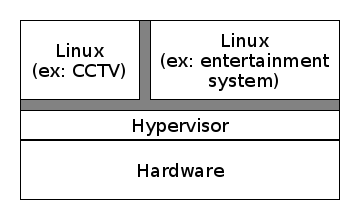
\includegraphics[height=4cm]{figures/figure-hypervisor-simple.png}
	\centering
	\caption{Two Linux on top of an hypervisor. They run isolated from each other and from the hypervisor.}
	\label{figure-hypervisor-simple}
\end{figure}

Previous work in the {prosper} project achieved to formally verify a simple separation kernel \cite{noauthor_prosper:_nodate-1,dam_formal_2013}, which later resulted into an implementation of a working hypervisor. Then, they achieved to run both Linux and {FreeRTOS} on top of it. Finally, they formally verified memory isolation for virtualized applications \cite{nemati_trustworthy_2015}. Nowadays, among other projects, the PROSPER team is working on device virtualization, allowing to give access to hardware devices to virtualized applications. An interesting example are {NIC} devices, which enable network communication and give the ability to communicate through the Internet.

A formal model of a {NIC} device has already been produced, on which some security theorems have been proved \cite{haglund_formal_2016}. These theorems can be seen as high-level proofs relying on a layer of lower-level lemmas. This layer provides an abstraction over the raw formal model. This is illustrated in the left-hand side of Figure \ref{hol-v-bir-nic-model-simple}.

\begin{figure}[H]
	\includegraphics[height=6cm]{figures/hol-v-bir-nic-model-simple.png}
	\caption{HOL4 v. BIR NIC models. The left hand side already exists. This project consists in the dashed elements. The dotted lines represent the work done during this project.}
	\label{hol-v-bir-nic-model-simple}
\end{figure}

The team is now developing a new framework for performing binary analysis in HOL4, an interactive theorem prover, named {holba} \cite{noauthor_holba_2019}. This framework is based on two papers written in the team. The first one introduces sound {transpilation} from binary to machine-independent code \footnotemark \cite{metere_sound_2017}. The second paper, ``TrABin: Trustworthy Analyses of Binaries'' \cite{lindner_trabin:_2019}, lays the foundations of the {holba} platform: it formally models {BIR}, introduces various supporting tools, implements two {proof-producing} {transpilers} (ARMv8 and Cortex-M0) and a proof-producing weakest precondition generator for loop-free programs.

\footnotetext{The machine-independent language used in the work is an implementation of {bap}'s BIL \cite{noauthor_binary_2019}. This implementation will evolve later in \cite{lindner_trabin:_2019} into BIR that HolBA uses today.}

While this kind of {transpilers} and {proof-producing} weakest precondition tools already exist \footnote{See related discussion in \cite{lindner_trabin:_2019}.}, the novelty in this work is that the transpiler is proof-producing, i.e. it produces a formal proof that both binary representations are equivalent, under the simulation theory, with respect to the {ISA} model. With this method, you no longer need to trust the transpiler. Figure \ref{holba-overview} gives an overview of the HolBA framework\footnote{TrABin works with both ARMv8 and Cortex-M0 binary programs. Only ARMv8 is showed in Figure \ref{holba-overview} to save some space.}.

\begin{figure}[H]
	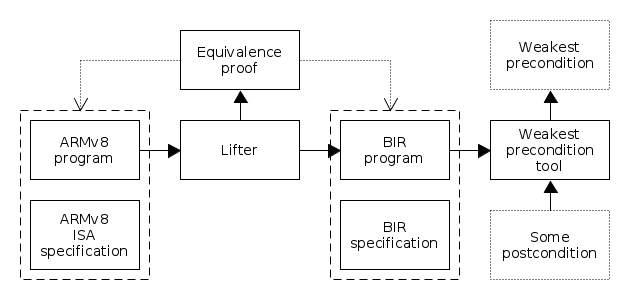
\includegraphics[height=5cm]{figures/holba-overview.png}
	\centering
	\caption{The HolBA framework. The lifter generates a BIR program and an equivalence proof from an ARMv8 program. The equivalence proof establishes a simulation property between the ARMv8 binary program and the generated BIR binary program, showing that they have the same behavior with respect to the ARMv8 {ISA} specification and the BIR specification. HolBA also support the Cortex-M0 ISA.}
	\label{holba-overview}
\end{figure}

The idea of this work is to translate the formal {NIC} model of \cite{haglund_formal_2016} using {BIR}, then use HolBA's proof-producing weakest precondition tool to prove the same lower-level lemmas than the formal model. With all the lemmas proved, the security properties are implied. Figure \ref{hol-v-bir-nic-model-simple} gives an overview of this idea: using the proof-producing weakest precondition tool to bind together a newly written BIR NIC model and the work done on the formal model.

\section{Intended readers}

In this thesis, formal verification is the central topic. The thesis presents how to model a hardware device using a binary analysis platform and presents some formal verification techniques. A reader interested in this topic may find the results presented useful for further work. A casual reader will be presented with a light introduction to the concepts that are essential in order to understand the problem that this thesis aims to explore. Those concepts should also be useful in order to understand software verification in general. For a more coherent reading, the concepts are introduced throughout the document. However, the reader is expected to have a background in Computer Science in general, and knowledge in formal verification will make the thesis easier to digest.

\section{Thesis objective}

The primary goal of this thesis project is to explore verification techniques in order to automate parts, if not all, of the verification process of hardware devices using the HolBA platform. The formal {NIC} model of \cite{haglund_formal_2016} is used as working example.

The ultimate goal would be to obtain a fully automatic pipeline for performing such verifications. However, it is evident that this goal isn't reachable in such a small amount of time, or even at all. Thus, this thesis focuses instead on exploring what toolkit is needed in order to facilitate this work.

\section{Delimitations}

This work being about the exploration of techniques towards automation of verification techniques, instead of being about producing an actual complete proof of a hardware device, some implementations have not been completed in order to save time to explore in more areas. Additionally, this work mainly concerns the HolBA platform that is developed in the team where this thesis took place.

\section{Choice of methodology}

This work has been carried out step-by-step toward an ideal goal, i.e. re-establishing all the security properties. On the road, needs have been identified and tools have been implemented in order to tackle them. This approach made sense in this particular work because the needs were not known in advance, and therefore needed to be identified. This thesis presents the steps taken during this work, the motivations of each tool that have been implemented, and discusses their limitations and future work in the conclusion.

%\end{multicols}
\end{document}























